%! Author = alida
%! Date = 18/12/2024

% Preamble
\documentclass[../main.tex]{subfiles}

% tutti i pacchetti usati vanno nel main

% Document
\begin{document}

    \section{Analisi}\label{sec:analisi}
%    \subfile{../../relazione/images}
        Nella fase di analisi, è stato effettuato un fit lineare ai dati
        appartenenti alla regione attiva delle caratteristiche in
        uscita, riportati nelle
        Tabelle~\ref{tab:100uA}~e~\ref{tab:200uA}.
        Per la precisione, al fine di ricavare i parametri
        desiderati direttamente dal fit, questo è stato eseguito
        con la funzione
        \begin{equation*}
            y = g \cdot ( x - V_A)
        \end{equation*}
        dove $g$ è la pendenza della retta, mentre $V_A$ rappresenta
        l'ascissa dell'intercetta con l'asse X.

        \begin{figure}[h!]
            \centering
            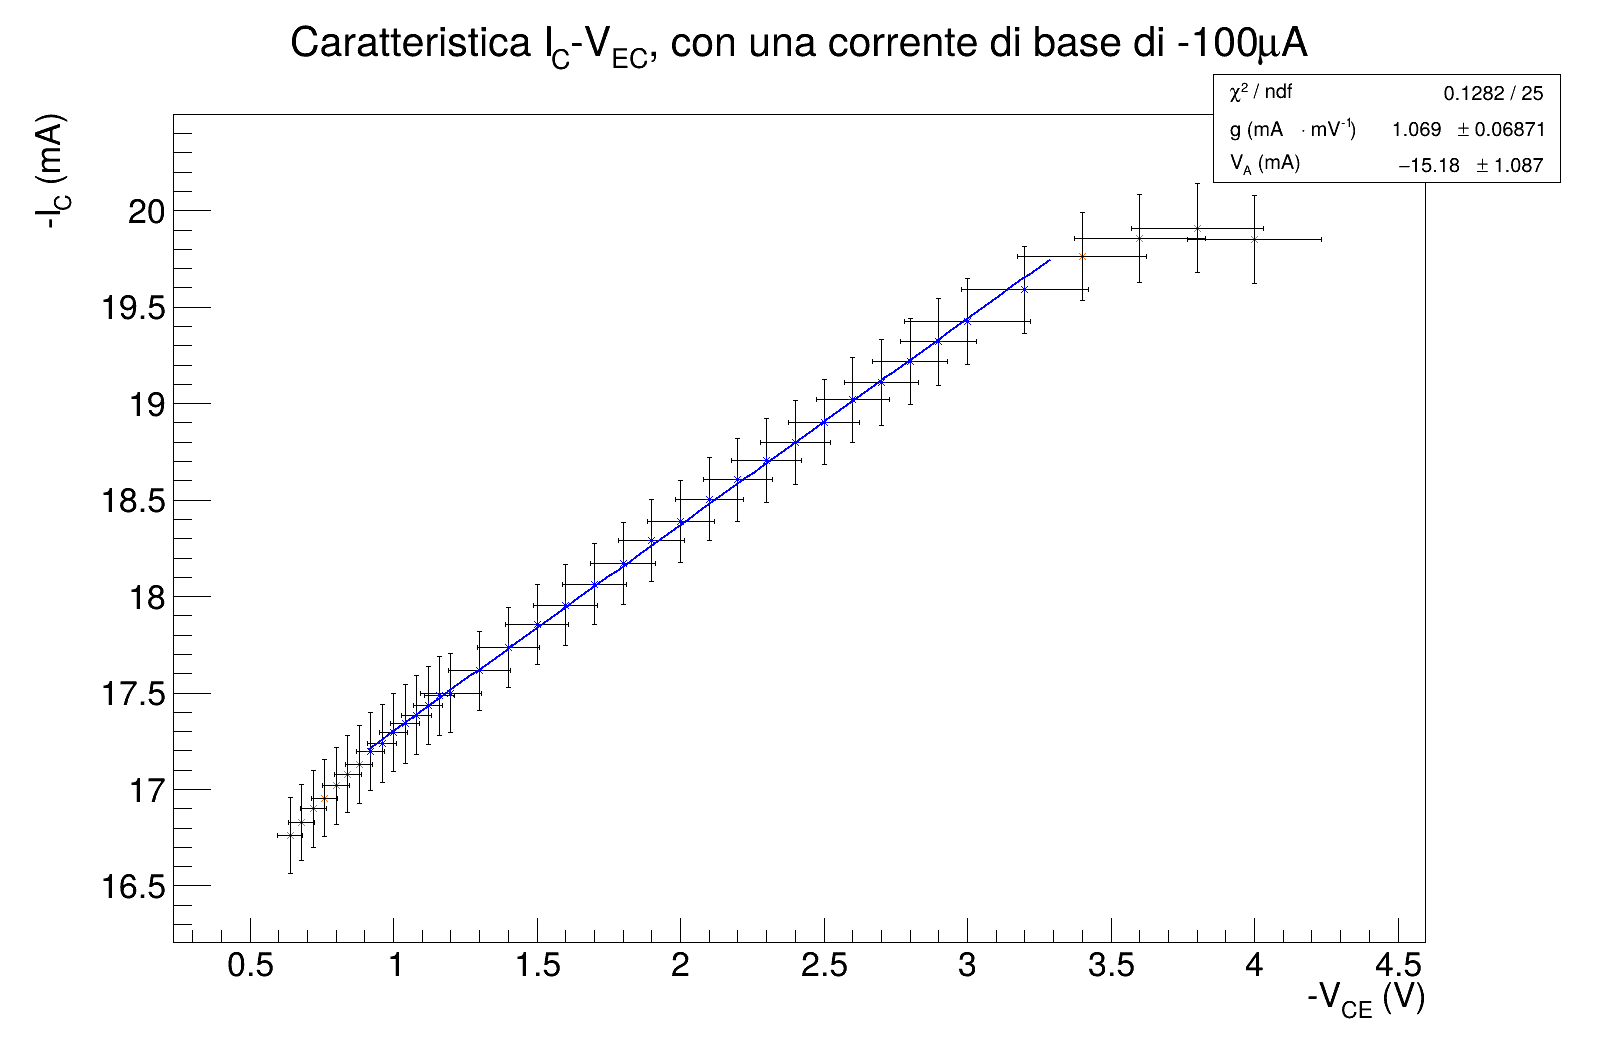
\includegraphics[width=.69\textwidth]{../../images/caratteristica-100uA}
            \caption{
                Grafico della caratteristica $I_C - V_{CE}$ ad assi
                invertiti e fit della regione attiva, con una
                corrente di base pari a $-100$ \textmu A.
            }
            \label{fig:fit-100}
        \end{figure}
        \begin{figure}[h!]
            \centering
            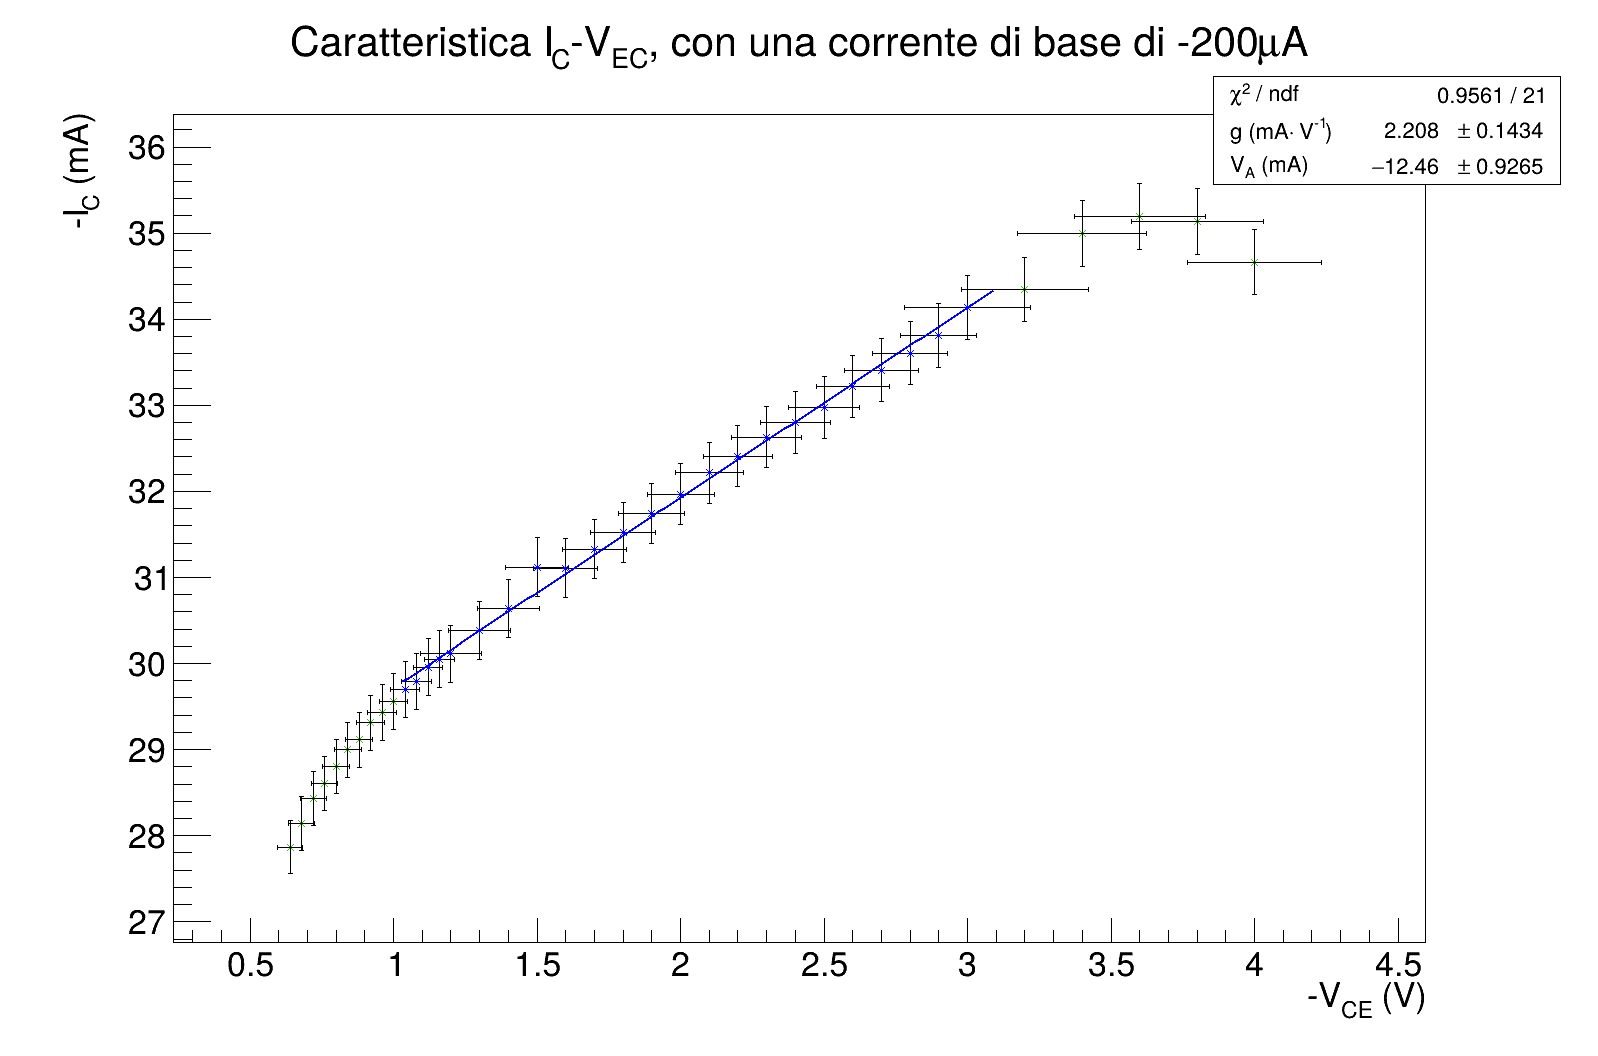
\includegraphics[width=.69\textwidth]{../../images/caratteristica-200uA}
            \caption{
                Grafico della caratteristica $I_C - V_{CE}$ ad assi
                invertiti e fit della regione attiva, con una
                corrente di base pari a $-200$ \textmu A.
            }
            \label{fig:fit-200}
        \end{figure}
        I risultati dei fit riportati nelle
        Figure~\ref{fig:fit-100}~e~\ref{fig:fit-200} e il valore
        della resistenza in uscita $b$ calcolato a partire da essi secondo
        l'Eq.\,\eqref{eq:g/b}, sono rispettivamente:

    \begin{table}[ht]
        \centering
        \begin{subtable}[t]{.45\textwidth}
            \centering
            \begin{tabular}{||c|c||}
                \hline
                \multicolumn{2}{||c||}{Corrente di base di -100~\textmu A} \\
                \hline
                \rule{0pt}{3ex} $V_A$ (V) & $15.2 \pm 1.1$ \\[1ex]
                \hline
                \rule{0pt}{3ex} $g$ (mA$\cdot$V$^{-1}$) & $1.069 \pm 0.069$ \\[1ex]
                \hline
                \rule{0pt}{3ex} $b$ (V$\cdot$mA$^{-1}$) & $0.935 \pm 0.060$ \\[1ex]
                \hline
            \end{tabular}
            \caption{-100 \textmu A}
            \label{tab:fit-100uA}
        \end{subtable}
        \hfill
        \begin{subtable}[t]{.45\textwidth}
            \centering
            \begin{tabular}{||c|c||}
                \hline
                \multicolumn{2}{||c||}{Corrente di base di -200~\textmu A} \\
                \hline
                \rule{0pt}{3ex} $V_A$ (V) & $12.46 \pm 0.93 $ \\[1ex]
                \hline
                \rule{0pt}{3ex} $g$ (mA$\cdot$V$^{-1}$) & $2.21 \pm 0.14$ \\[1ex]
                \hline
                \rule{0pt}{3ex} $b$ (V$\cdot$mA$^{-1}$) & $0.453 \pm 0.029$ \\[1ex]
                \hline
            \end{tabular}
            \caption{-200 \textmu A}
            \label{tab:fit-200uA}
        \end{subtable}

        \vspace{0.5pt} % Spazio opzionale tra minipage e caption generale

        \caption{Risultati dei fit lineari effettuati sulle misure delle caratteristiche in uscita del transistor BJT,
            corrispondenti a una corrente di base di (a) -100\;\textmu A, (b) -200\;\textmu A, e valori della
            resistenza calcolati a partire da essi.}
        \label{tab:fit_caratteristiche}

    \end{table}

    \begin{figure}[h!]
        \centering
        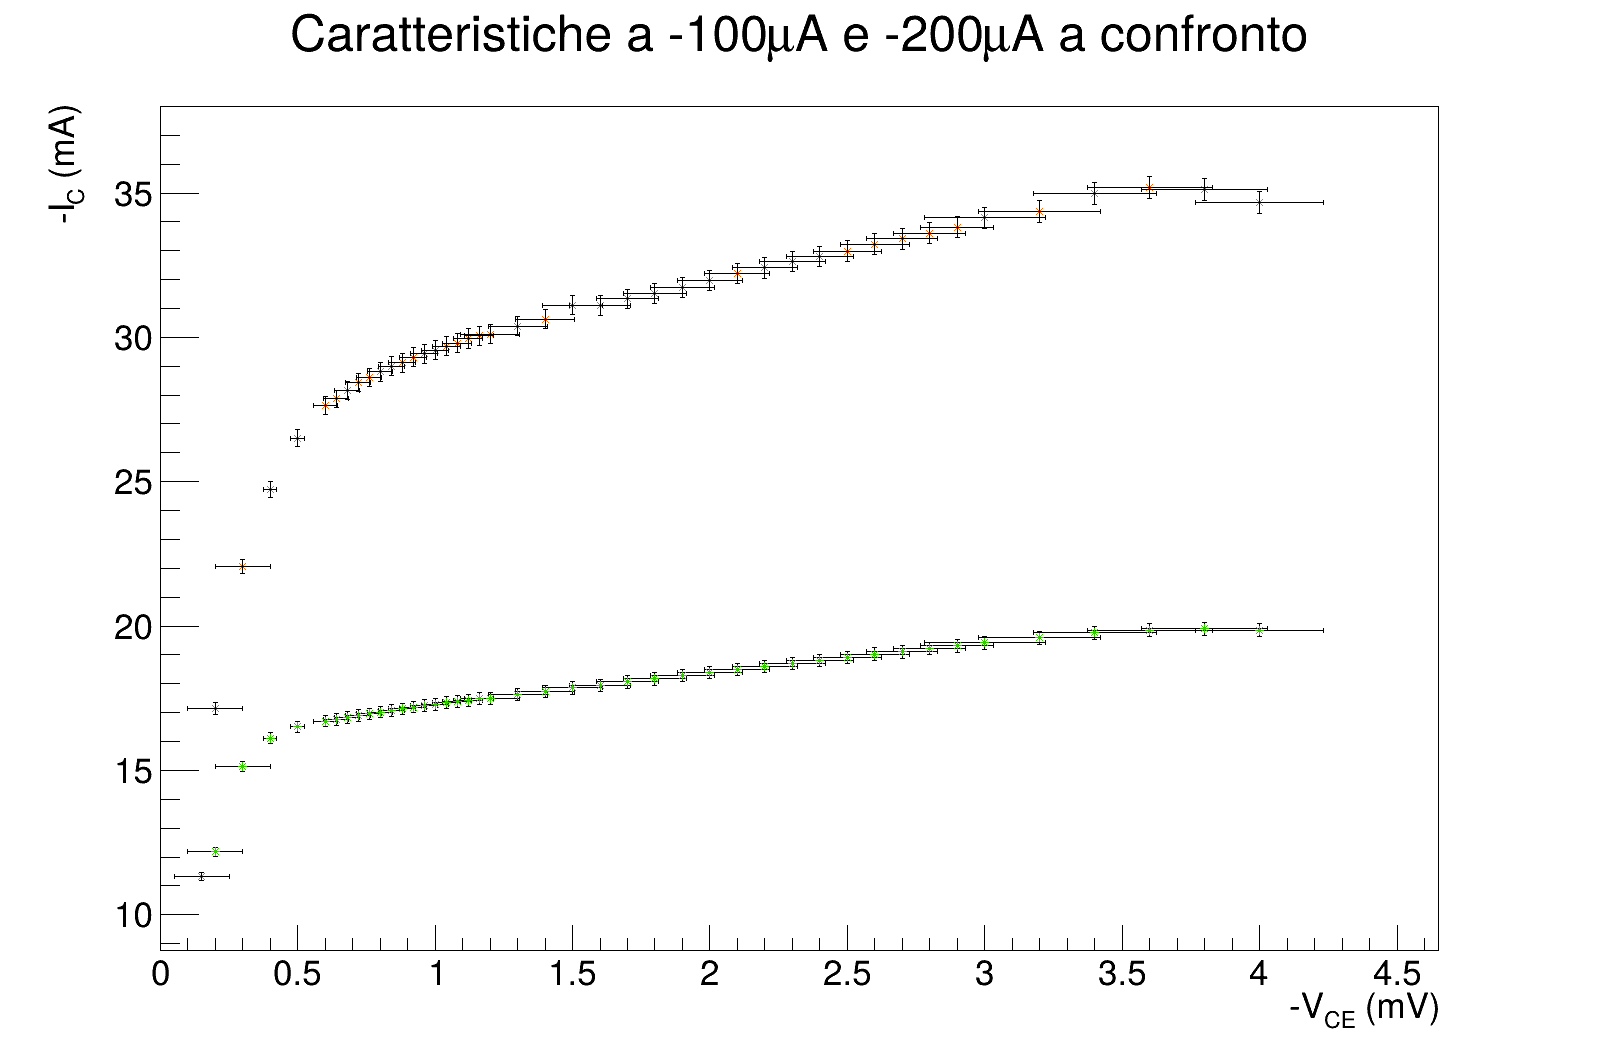
\includegraphics[width=.8\textwidth]{../../images/caratteristiche-confronto}
        \caption{Grafico delle carateristiche a $-100$~\textmu A e $-200$~\textmu A a confronto.}
        \label{fig:aggregato}
    \end{figure}

    \noindent Infine si è calcolato il guadagno di corrente $\beta(V_{CE})$ definito come:
    \begin{equation*}
        \beta(V_{CE}) = \frac{\varDelta I_C(V_{CE})}{\varDelta I_B} = \frac{\varDelta I_C(V_{CE})}{0.1}
    \end{equation*}

    \begin{figure}[h!]
        \centering
        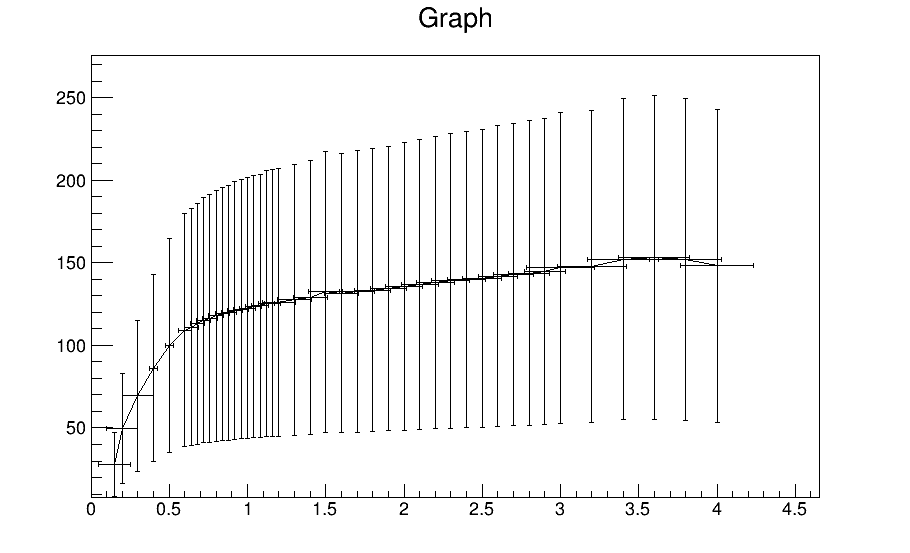
\includegraphics[width=0.7\textwidth]{../../images/beta}
        \caption{
            Grafico del guadagno di corrente $\beta$ tra le
            caratteristiche a -100~\textmu A e -200~\textmu A, in
            funzione di $V_{CE}$.
        }
        \label{fig:beta}
    \end{figure}
    \noindent È immediato notare l'entità degli errori sui valori di $\beta$
    riportati nel grafico in Figura~\ref{fig:beta}, per la
    spiegazione si veda l'appendice~\ref{sec:errori-beta}.
    Tra i punti nel grafico si riporta esplicitamente il valore:
    \begin{center}
        $\beta(-2) = 136 \pm  87$
    \end{center}


\end{document}